\section{Node Design}
\label{sec:node}
The \bus defines two {\em physical} types of nodes: member nodes and a
mediator node. An instantiation of \bus must have one and only one mediator
node and must have at least one member node (N$\geq$1). The maximum number of
member nodes is a function of clock speed\footnote{
  The maximum chip-to-chip latency is defined as 10~ns. Assuming a TX node has
similar delay to generate the next bit and clock delay to nodes is 0, then the
minimum cycle time is N nodes * 20~ns. \bus designers are obligated to
consider all possibly delays and thus define a maximum feasible clock speed,
however, for most designs the maximum clock speed theoretically possible will
largely exceed the plausible speed for the given power budget.}.

During a transmission, \bus defines three {\em logical} types of nodes:
a transmitting node, a receiving node, and forwarding nodes. During a
transmission, there must be exactly one transmitting and one receiving node.
Any number (N$\geq$0) of forwarding nodes are permitted.

%%%%%%%%%%%%%%%%%%%%%%%%%%%%%%%%%%%%%%%%%%%%%%%%%%%%%%%%%%%%%%%%%%%%%%%%%%%%%%%%
\subsection{Physical Design}
\label{sec:physical}

From a package perspective, the physical design of a member and mediator node
is the same, each must expose a {\tt DIN}, {\tt DOUT}, {\tt CLKIN} and {\tt
CLKOUT} pad.

In addition, one (or more?) chip(s) on the bus can add two additional pads to
act as a ``splitter'' node, to allow the interjection of new devices on the
bus. This part of \bus is not yet well-defined.

\subsubsection{Member Nodes}
\label{sec:physical-member}
A member node requires 4 signals:

\begin{itemize}
  \item {\tt DIN} -- Data In
  \item {\tt DOUT} -- Data Out
  \item {\tt CLKIN} -- Clock In
  \item {\tt CLKOUT} -- Clock Out
\end{itemize}

Most of the time, a member node is in the {\sc forwarding} state. While
forwarding, a member node must amplify and forward signals from the {\tt DIN}
pin to the {\tt DOUT} pin and from the {\tt CLKIN} pin to the {\tt CLKOUT} pin.
Designs should attempt to minimize latency between these pins. The maximum
propagation latency\footnote{
  The amount of time taken to propagate a change in the output of the {\em
  previous} link in the data loop to the output of the next link in the data
  loop. This time includes all of the internal forwarding logic from {\tt DIN}
  to {\tt DOUT} or {\tt CLKIN} to {\tt CLKOUT}, as well as any pin/wire
  capacitance that must be overcome to drive the next input gate.
  }
permitted is 10~ns. \bus defines a maximum load capacitance of \hl{XXX}~pF for
the {\tt DIN} pin and of \hl{XXX}~pF for the {\tt CLKIN} pin to enable
inter-operability of generalized components\footnote{
  However, the only strict requirement is the 10~ns propagation delay, thus
  careful designers may violate this requirement if necessary.
  }.

\subsubsection{Mediator Node}
\label{sec:physical-mediator}
A mediator node requires 4 signals:

\begin{itemize}
  \item {\tt DIN} -- Data In
  \item {\tt DOUT} -- Data Out
  \item {\tt CLKIN} -- Clock In
  \item {\tt CLKOUT} -- Clock Out
\end{itemize}

While forwarding, the mediator node is subject to the same propagation latency
constraints (10~ns) as member nodes.


\subsubsection{Bus Connections}
\label{sec:physical-bus}
\begin{itemize}
  \item {\tt DIN}, {\tt DOUT}
  \begin{itemize}
    \item The data pins shall be connected in a round-robin fashion, the
      {\tt DOUT} of one chip connected to the {\tt DIN} of the next.
    \item The connection of data lines must form a loop when connected
      correctly (e.g.~\cref{fig:bus}).
    \item There are no requirements for the placement of nodes in the data
      loop, but the ordering will have an impact on bus arbitration. See
      \cref{sec:bus-arbitration} for more details.
  \end{itemize}
  \item {\tt CLK}
  \begin{itemize}
    \item The clock pins shall be connected in a round-robin fashion. The
      {\tt CLKOUT} of one chip connected to the {\tt CLKIN} of the next.
    \item The connection of clock lines must form a loop when connected
      correctly (e.g.~\cref{fig:bus}).
    \item The connection of clock lines must match that of data lines. That
      is, if a node N$_{a}$ connects its {\tt DOUT} to the {\tt DIN} of node
      N$_{b}$, the {\tt CLKOUT} of N$_{a}$ must be connected to the {\tt DIN}
      of N$_{b}$.
  \end{itemize}
  A \bus must have a minimum of two nodes (one mediator node and one
  member node). Single chips that are not connected to a bus should tie
  {\tt CLKIN} and {\tt DIN} high and leave {\tt CLKOUT} and {\tt DOUT}
  floating.
\end{itemize}


\subsubsection{Injection}
Injection is the ability for an arbitrary additional node to temporarily (or
permanently) interpose itself into a \bus instantiation. Two examples are a
system programmer or a debugger.

The exact method of injection is not defined by \bus. It may be as simple as
exposing a pair of out/in pins that are normally jumpered, some packages may
not have such luxury. Injection is mentioned here as it is an exceptionally
useful tool for system bring-up and development. The means for performing
injection should be considered as a \bus instantiation is designed.


%%%%%%%%%%%%%%%%%%%%%%%%%%%%%%%%%%%%%%%%%%%%%%%%%%%%%%%%%%%%%%%%%%%%%%%%%%%%%%%%
\subsection{Logical Design}
\label{sec:logical}

There are three {\em logical} types of \bus nodes: transmitting, receiving,
and forwarding. \bus can be considered multi-master, any node is capable of
transmitting to any other node. The mediator node adopts these same three
personalities, but its behavior differs slightly during
arbitration~(\ref{sec:bus-arbitration}).

\begin{figure}
  \begin{minipage}[b]{.48\linewidth}
    \centering
    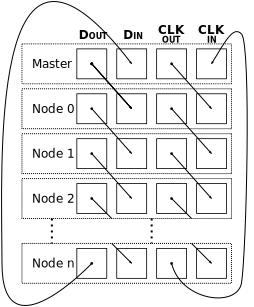
\includegraphics[width=0.5\linewidth]{img/stacked_layers}
    \caption{\textbf{\bus Physical Topology.} \textmd{
        High-level picture of \bus physical design. Member nodes and a
        mediator node are connected in a loop, with data and clock lines
        forming independent rings.
    }}
    \label{fig:bus}
  \end{minipage}
  \hspace{1 em}
  \begin{minipage}[b]{.48\linewidth}
    \centering
    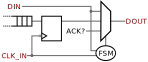
\includegraphics[width=\textwidth]{img/logical}
    \caption{\textbf{Logical Model.} \textmd{
        The Finite State Machine selects between the three modes a node can be
        in. Top: {\em forwarding}, Mid: {\em transmitting}, Bot: {\em
        acknowledging}. This model omits some of the subtleties of
        arbitration,
        see~\ref{sec:state-arbitrate}~\nameref{sec:state-arbitrate} for
        details.
    }}
    \label{fig:logical}
  \end{minipage}
\end{figure}

\begin{figure}[h]
  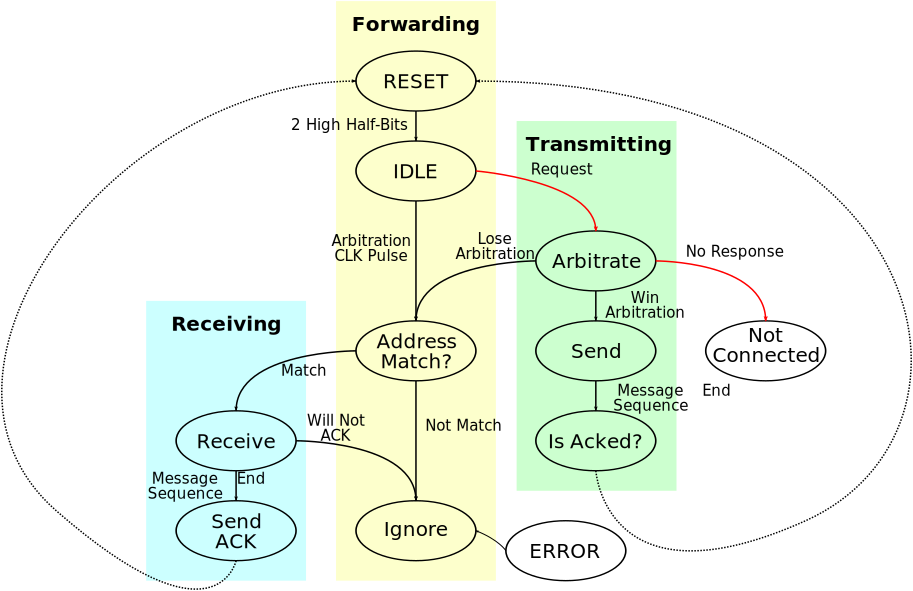
\includegraphics[width=\linewidth]{img/fsm_diagram}
  \caption{\textbf{FSM describing the high-level logical behavior of \bus
    nodes.} \textmd{
    Black arrows indicate transitions that occur on bus clock edges. Not shown
    are implicit arrows from any state to Forwarding.{\sc control}. From any
    {\sc control} state, nodes progress to {\sc idle}.
    }}
\end{figure}

\subsubsection{Forwarding}
Forwarding is the most common state for all \bus nodes. Observe in
\autoref{fig:logical} the very simple, short logic path from {\tt DIN} to
{\tt DOUT}. Nodes are obligated to forward data in less than 10~ns.

\paragraph{Forwarding.\textsc{Idle}}
This is the rest/idle state for \bus nodes. In this state member nodes may be
completely power-gated and asleep. The only obligation is that {\tt DIN} is
forwarded to {\tt DOUT} and {\tt CLKIN} is forwarded to {\tt CLKOUT}.

\medskip
\noindent
{\em Mediator Node Exception:} In \textsc{idle}, the mediator node does not
forward {\tt DIN} to {\tt DOUT}.

\paragraph{Forwarding.\textsc{Address\_Match}}
At the start of a new transmission, a forwarding node should monitor the {\tt
DIN} line to see if it is the target for this transmission. If a node matches
its address, it promotes itself from forwarding to receiving. After the first
mis-matched bit a forwarding node transitions to the {\sc ignore} state for
the rest of the transaction.

\paragraph{Forwarding.\textsc{Ignore}}
In {\sc ignore} nodes simply forward data. Nodes remain in this state until
an interjection. Power-conscious designs may safely power gate everything
except interjection detector circuitry while in {\sc ignore}.

\subsubsection{Transmitting}

\paragraph{Transmitting.{\sc arbitrate}}
\label{sec:state-arbitrate}
A node initiates a transmission by pulling its {\tt DOUT} line low. A node may
only attempt to initiate a transmission while the bus is idle. Care must be
taken in detecting the bus idle state when requesting to transmit. In
particular, a node requesting to transmit must ensure that the {\tt CLK} line
is still high, it is not sufficient to rely on the local state machine still
being in the {\sc idle} state\footnote{To envision the case defended against
here, picture a tall stack of nodes, where the bottom node requests the bus.
The mediator node pulls {\tt CLK} low in response. Shortly before the mediator
node pulls {\tt CLK} high, a node at the top of the stack (still in the {\sc
idle} state) elects to transmit. There is not enough time for his {\tt DOUT}
to propagate to the bottom node, however, thus when {\tt CLK} goes high, both
the bottom and top nodes believe they have won the arbitration. Designers must
select a sufficiently long period $t_{long}$ to ensure all signals are stable.
Twice the maximum possible propagation delay (delay for falling {\tt CLK} to
furthest node + furthest node's {\tt DOUT} back to closest node) of the system
should be sufficient.}.

The {\sc arbitrate} state is left when the {\tt CLK} line is pulled high by
the mediator node. If a member node's {\tt DIN} is high on the rising clock
edge, it has won arbitration. A node that loses arbitration should begin
listening to see if it is the destination node. If the {\tt CLK} line never
goes high---where never is defined as four times the minimum clock speed of
\bus\footnote{\hl{TODO: TBD}}---the node should consider itself as
disconnected.

Details of priority arbitration are omitted here for simplicity.
See~\ref{sec:bus-arbitration}~\nameref{sec:bus-arbitration} for
details.

\medskip
\noindent
{\em Mediator Node Exception:} The mediator node always wins arbitration. Note
that when this occurs, the mediator node's {\tt DIN} will be low.

\medskip
\noindent
{\em Mediator Node Exception:} If a mediator node pulls its {\tt DOUT} line low
and its {\tt DIN} line never goes low, it should be considered
{\sc Not\_Connected}.

\paragraph{Transmitting.{\sc send}}
During {\sc send}, a transmitting node pushes bits onto the bus as described
in~\ref{sec:bus-transmission}~\nameref{sec:bus-transmission}.

A transmitting node completes its transmission by interjecting
(\ref{sec:bus-interjection}~\nameref{sec:bus-interjection}) the bus
and indicating the transmission is complete.

\paragraph{Transmitting.{\sc control}}
As a transmitter, a node is responsible for the first control bit. This bit
should be set by a transmitter to indicate that the complete message has been
sent. The transmitter must listen to the subsequent control bits to establish
if the message was acknowledged and if the targeted layer is sending a
response.

\subsubsection{Receiving}

\paragraph{Receiving.{\sc Receive}}
A receiving node is also obligated to forward data along the bus. In the
sketch shown in \cref{fig:logical}, during the receiving process, a
receiving node remains in pass-thru mode until an interjection.

\paragraph{Receiving.{\sc control}}
A receiver must acknowledge the successful receipt of a transmission. If a
receiver wishes to NAK a transmission, it simply does nothing during the
ACK/NAK control bit.

A receiver may also possibly enter control by electing to interject the bus
itself. A receiver will interject a transmission to indicate that its RX
buffer has been overrun and the current transmission must be aborted.

\subsubsection{Exception States}

\paragraph{Exception.{\sc Not\_Connected}}
A robust implementation should include detection of some kind for an attempt
to utilize the bus when the node is not actually connected to a bus (so that
it may report failure). After a node pulls its {\tt DOUT} low there is a
maximum possible $t_{long}$ of \hl{TODO} before a mediator node must pull
{\tt CLK} low in response. If {\tt CLK} is not pulled low, the node should
consider itself disconnected and report failure to send as appropriate.
